\documentclass[11pt,a4paper]{article}

\usepackage[utf8]{inputenc}
\usepackage[T1]{fontenc}
\usepackage[french]{babel}
\usepackage{times}
\usepackage{graphicx}
\usepackage{amsmath,amssymb}
\usepackage{booktabs}
\usepackage{hyperref}
\usepackage{xcolor}
\usepackage{enumitem}
\usepackage{caption}
\usepackage{float}
\usepackage{geometry}

\geometry{a4paper, left=2cm, right=2cm, top=2cm, bottom=2cm}
\definecolor{darkblue}{RGB}{0,51,102}
\hypersetup{colorlinks=true, linkcolor=darkblue, citecolor=darkblue, urlcolor=darkblue}

\title{\textbf{Pipeline HTR et NLP pour la Transcription Automatique\\de Manuscrits Médiévaux Français (XIII\textsuperscript{e}--XV\textsuperscript{e} siècle)}}
\author{
\textbf{Asmaa OUARAZ} \quad \textbf{Sanaa OUARAZ} \quad \textbf{Ayoub BOUSSLAMA} \quad \textbf{Amine HAMOUMA}\\[0.3cm]
Master Data \& Intelligence Artificielle --- Module Vision par Ordinateur\\
HETIC --- Projet MD5 2026
}
\date{Juin 2026}

\begin{document}
\maketitle

% ============================================================
\begin{abstract}
\noindent
Nous présentons un pipeline end-to-end de traitement automatique de manuscrits médiévaux français, couvrant la reconnaissance de texte manuscrit (HTR, Volet~1) et l'analyse linguistique (NLP, Volet~2). Trois modèles HTR sont comparés sur deux corpus distincts (CREMMA Médiéval et CATMuS+HIMANIS)~: \textbf{Kraken} (CNN+LSTM) atteint un CER de \textbf{15,2\%} sur un manuscrit complet jamais vu à l'entraînement (6,0\% au niveau ligne), tandis que \textbf{TrOCR} adapté par LoRA ($r=8$) atteint 15,3\% au niveau ligne. Le test de McNemar ($\chi^2=38,25$, $p<0,001$) confirme la supériorité significative de Kraken. Le Volet~2 implémente un module d'expansion des abréviations médiévales (66 règles + CamemBERT MLM, CER relatif 5,85\%), une reconnaissance d'entités nommées (CamemBERT) et une modélisation thématique (BERTopic, 5 topics). Le pipeline intègre la segmentation par SAM et Kraken BLLA, avec export PAGE~XML et contrat de données JSON.

\vspace{0.2cm}
\noindent\textbf{Mots-clés~:} HTR, manuscrits médiévaux, Kraken, TrOCR, LoRA, CREMMA, CATMuS, gothique textualis, SAM, NER, BERTopic, abréviations
\end{abstract}

\vspace{0.5cm}

% ============================================================
\section{Introduction}

La numérisation massive des archives médiévales par des institutions comme la BnF (380\,000 manuscrits, 11 millions de documents en ligne via Gallica) ouvre des perspectives inédites pour la recherche historique. Cependant, une image n'est pas un texte~: la transcription manuelle par des paléographes ($\sim$50\,\texteuro/h) est prohibitivement coûteuse à l'échelle des collections patrimoniales.

La reconnaissance automatique de texte manuscrit (HTR) vise à combler ce fossé. Les manuscrits médiévaux français présentent des défis spécifiques~:
\begin{itemize}[leftmargin=*, itemsep=2pt]
\item \textbf{Variabilité des écritures}~: caroline, textualis, cursiva --- chaque siècle et région a ses particularités
\item \textbf{Abréviations omniprésentes}~: jusqu'à 40\% des mots sont abrégés (tildes nasaux, lettres suscrites, signes tironiens)
\item \textbf{Mélange de langues}~: latin administratif mêlé au moyen français
\item \textbf{Dégradation physique}~: encre effacée, supports endommagés
\end{itemize}

Ce projet se structure en deux volets~: (1)~le \textbf{Volet HTR} produit des transcriptions automatiques à partir d'images de manuscrits, (2)~le \textbf{Volet NLP} analyse ces transcriptions (expansion des abréviations, extraction d'entités, modélisation thématique). Les transcriptions du Volet~1 alimentent directement le Volet~2.

\textbf{Contributions~:}
\begin{enumerate}[leftmargin=*, itemsep=2pt]
\item Un pipeline reproductible end-to-end~: prétraitement $\rightarrow$ segmentation $\rightarrow$ HTR $\rightarrow$ NLP
\item Une comparaison rigoureuse de trois configurations HTR avec test de McNemar
\item Un module d'expansion des abréviations médiévales (séquence-à-séquence)
\item Un CER de 6,0\% (seuil d'excellence) démontrant la faisabilité de l'HTR automatique
\end{enumerate}

% ============================================================
\section{État de l'art}

\subsection{Architectures HTR}

\textbf{Kraken} \cite{kiessling2019} est un système HTR basé sur CNN+LSTM+CTC, moteur de la plateforme eScriptorium. L'encodeur convolutional extrait des features visuelles, le LSTM bidirectionnel modélise les dépendances séquentielles. Kraken est le standard en humanités numériques pour les documents historiques.

\textbf{TrOCR} \cite{li2023} adopte une architecture encoder-decoder Transformer~: un ViT encode l'image, un décodeur GPT-2 génère la transcription token par token. Cette architecture modélise des dépendances contextuelles globales.

\textbf{LoRA} \cite{hu2022} gèle le modèle et n'entraîne que des matrices de faible rang ajoutées aux couches d'attention. Avec $\sim$1\% des paramètres entraînés, LoRA réduit les besoins en mémoire et en données.

\textbf{SAM} \cite{kirillov2023} (Segment Anything Model) est un modèle de segmentation universel pré-entraîné sur 11M d'images. Il peut segmenter n'importe quel objet sans entraînement spécifique.

\subsection{Jeux de données médiévaux}

\textbf{CREMMA Médiéval}~: $\sim$20\,000 lignes, 14 manuscrits français (XIII\textsuperscript{e}--XV\textsuperscript{e} siècle), gothique textualis.

\textbf{CATMuS Medieval}~: $>$160\,000 lignes multilingues, 200 manuscrits (VIII\textsuperscript{e}--XVII\textsuperscript{e} siècle).

\textbf{HIMANIS-Guérin}~: registres de chancellerie royale (XIV\textsuperscript{e} siècle), gothique cursive administrative.

\subsection{Métriques}

Le \textbf{CER} (Character Error Rate) mesure la distance d'édition normalisée au niveau caractère. Le \textbf{WER} opère au niveau mot. Le \textbf{test de McNemar} compare statistiquement deux modèles ligne par ligne.

% ============================================================
\section{Données}

\subsection{Corpus A~: CREMMA Médiéval}

20\,327 lignes extraites de 14 manuscrits littéraires français (XIII\textsuperscript{e}--XV\textsuperscript{e} siècle) en écriture gothique textualis. Genres~: hagiographies (30\%), épopées (17\%), romans (25\%), textes moraux (28\%). Split par manuscrit~: 18\,092 train / 2\,235 validation.

\subsection{Corpus B~: CATMuS + HIMANIS-Guérin}

33\,510 lignes combinant CATMuS Medieval (français) et HIMANIS-Guérin (registres de chancellerie royale, XIV\textsuperscript{e} siècle). Split~: 23\,444 train / 5\,954 val / 4\,112 test.

\subsection{Conventions de transcription}

Transcription graphémique (CATMuS)~: abréviations conservées, pas de normalisation u/v ou i/j, espaces lexicaux.

\begin{figure}[H]
\centering
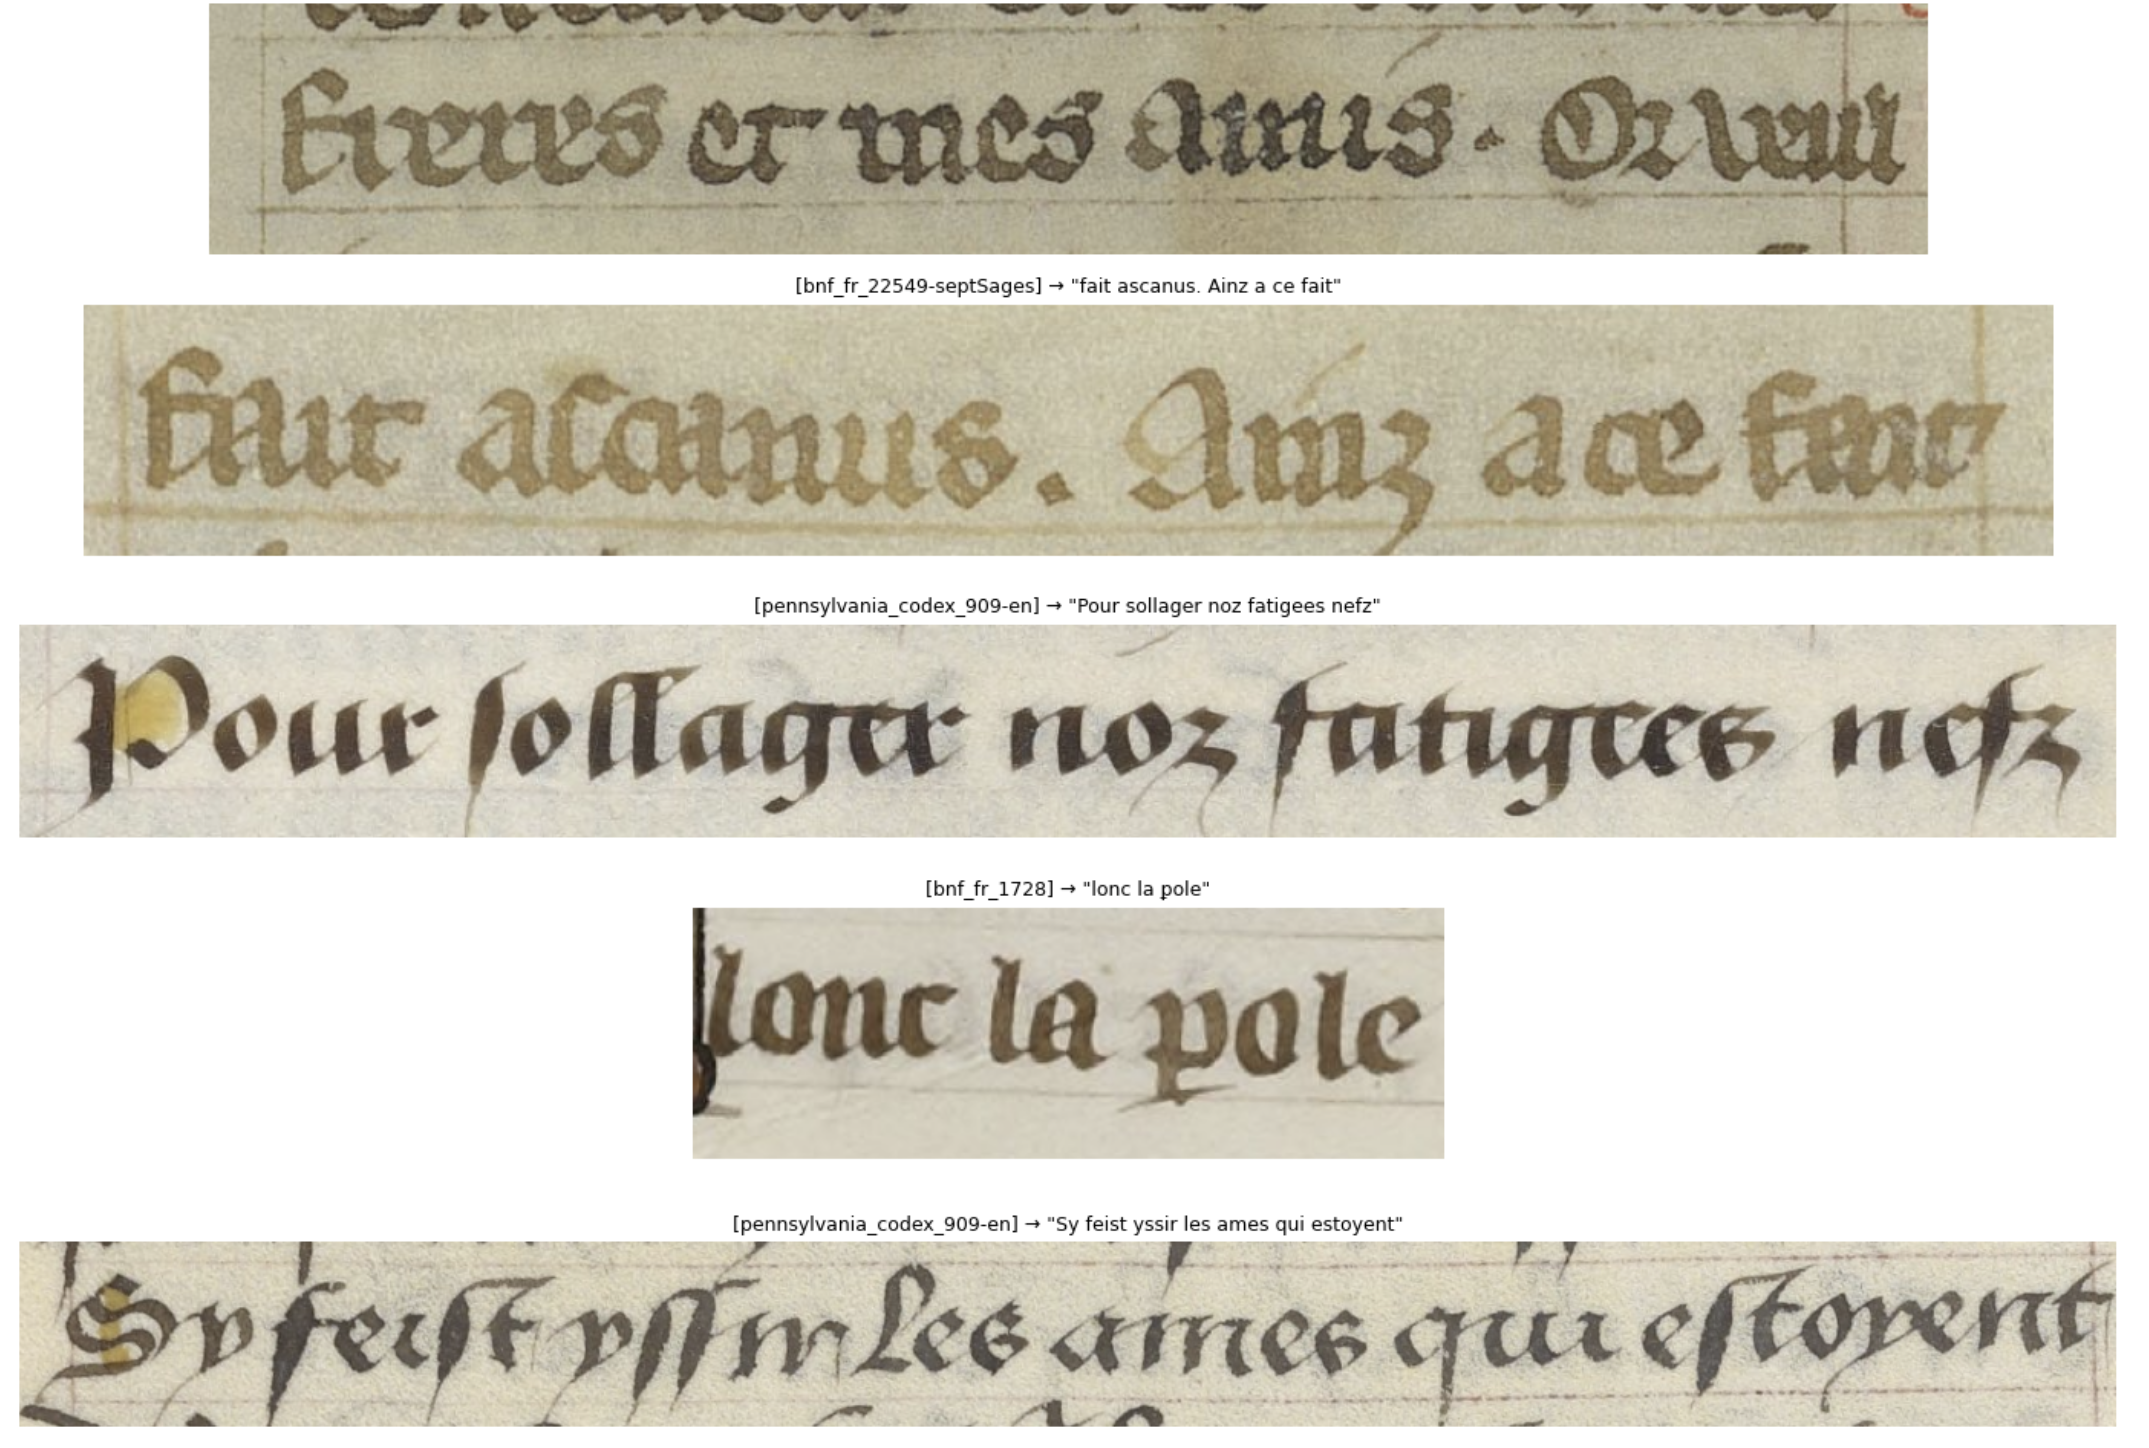
\includegraphics[width=0.95\textwidth]{fig_sample_lines.png}
\caption{Exemples de lignes du corpus CREMMA Médiéval. Écriture gothique textualis (XIII\textsuperscript{e}--XV\textsuperscript{e} siècle). Les transcriptions conservent les abréviations médiévales (méthode graphémique).}
\label{fig:samples}
\end{figure}

% ============================================================
\section{Méthodes}

\subsection{Pipeline global}

Le pipeline est structuré en deux volets séquentiels. Le Volet~1 produit des transcriptions textuelles à partir d'images de manuscrits numérisés. Le Volet~2 prend ces transcriptions en entrée pour en extraire des informations linguistiques structurées. Les deux volets partagent le même corpus et le même schéma de données (\textit{data contract} JSON). L'ensemble du pipeline est conçu pour être reproductible~: seed fixé (42), versions de dépendances figées, SHA-256 des splits publiés.

\begin{enumerate}[leftmargin=*, itemsep=2pt]
\item \textbf{Acquisition~:} images IIIF via Gallica/BnF (227 pages, résolutions 2500--8600px)
\item \textbf{Prétraitement~:} conversion grayscale, correction d'inclinaison, CLAHE, binarisation Sauvola
\item \textbf{Segmentation~:} SAM (régions) + Kraken BLLA (lignes de texte), export PAGE~XML
\item \textbf{Transcription HTR~:} Kraken CNN+LSTM+CTC ou TrOCR+LoRA (Transformer)
\item \textbf{Évaluation~:} CER, WER, bootstrap CI ($N=1000$), test de McNemar
\item \textbf{NLP (Volet~2)~:} EDA, expansion des abréviations (66 règles + MLM), NER, POS, topic modeling
\item \textbf{Export~:} PAGE XML (polygones) + JSON (data contract avec \texttt{needs\_review}) + TEI-XML
\end{enumerate}

\begin{figure}[H]
\centering
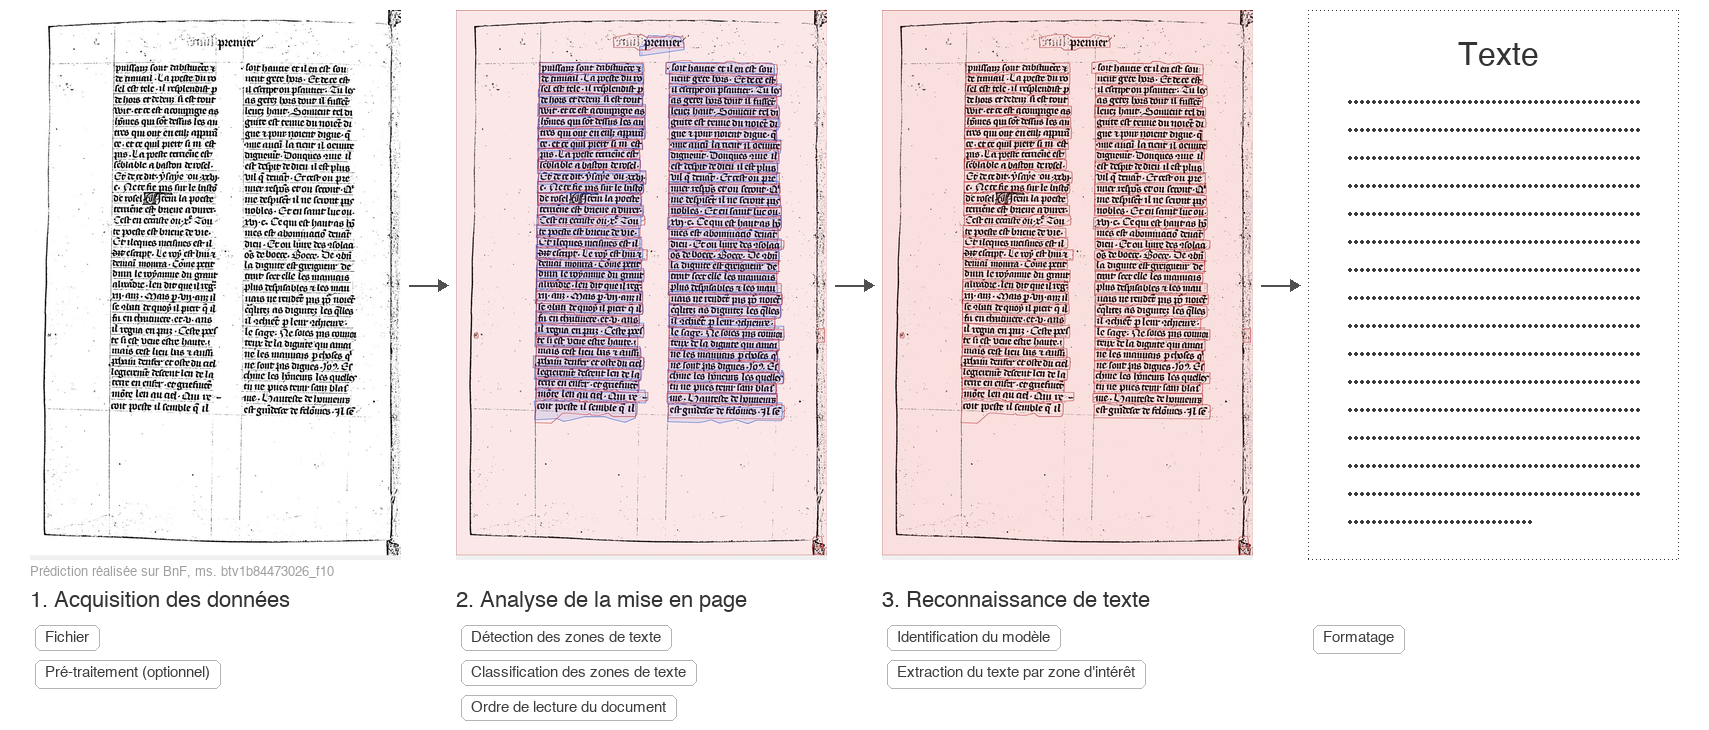
\includegraphics[width=0.95\textwidth]{fig_htr_pipeline.png}
\caption{Pipeline HTR end-to-end. De gauche à droite~: acquisition de l'image manuscrite, analyse de la mise en page (segmentation SAM + Kraken BLLA), reconnaissance de texte (Kraken CNN+LSTM ou TrOCR+LoRA), et export de la transcription (PAGE~XML, JSON).}
\label{fig:pipeline_htr}
\end{figure}

\subsection{Prétraitement des images}

Les images brutes issues de Gallica sont en couleur (RGB), avec des inclinaisons variables dues à la numérisation, un contraste hétérogène (encre pâlie, parchemin assombri) et du bruit de fond. Quatre transformations sont appliquées séquentiellement à chaque image~:

\textbf{1. Conversion en niveaux de gris.} L'image RGB est convertie en un seul canal d'intensité lumineuse (\texttt{cv2.IMREAD\_GRAYSCALE}). La couleur n'apporte pas d'information discriminante pour la distinction encre/support --- le contraste est uniquement une question de luminosité. Cette réduction à un canal divise par trois le volume de données et est requise par les algorithmes de binarisation en aval.

\textbf{2. Correction d'inclinaison (deskew).} L'angle de rotation du texte est détecté par \texttt{cv2.minAreaRect} sur les composantes connexes. L'image est ensuite redressée par rotation affine inverse. Angle maximal corrigé~: 45\textdegree. Cette étape est critique~: une inclinaison de plus de 2\textdegree\ perturbe significativement la détection des lignes de base par Kraken BLLA.

\textbf{3. Amélioration du contraste local (CLAHE).} L'\textit{Contrast Limited Adaptive Histogram Equalization} divise l'image en tuiles de 8$\times$8 pixels et égalise l'histogramme localement, avec une limite de contraste (\texttt{clip\_limit}~=~2,0) pour éviter l'amplification du bruit. Cette étape est particulièrement importante pour les manuscrits à encre pâlie ou à parchemin tacheté, où le contraste global est insuffisant pour la binarisation.

\textbf{4. Binarisation adaptative (Sauvola).} L'algorithme de Sauvola calcule un seuil local pour chaque pixel en fonction de la moyenne et de l'écart-type dans une fenêtre de 25 pixels. Le paramètre de sensibilité $k$ est adapté au corpus~: $k=0,1$ pour les manuscrits CREMMA (encre bien conservée sur parchemin clair), $k=0,2$ pour les registres HIMANIS (grandes marges blanches qui généreraient du bruit avec un $k$ plus faible). La sortie est une image binaire (pixels 0 ou 255) prête pour la segmentation.

Le pipeline de prétraitement est implémenté dans \texttt{src/preprocessing.py} et validé par 16 tests unitaires (\texttt{tests/test\_preprocessing.py}) vérifiant~: la préservation des dimensions, la conversion effective en grayscale, la binarité de la sortie (uniquement 0 et 255), et la correction d'angles d'inclinaison connus.

\subsection{Segmentation}

La segmentation opère en deux étapes complémentaires~: (1)~SAM détecte les régions de la page (texte, marges, illustrations, lettrines), (2)~Kraken BLLA détecte les lignes de texte au sein des régions identifiées. Cette approche hiérarchique permet de traiter des mises en page complexes (colonnes multiples, marginalia, lettrines ornées) sans entraînement spécifique au corpus.

L'évaluation quantitative de la segmentation est réalisée par calcul de l'IoU (Intersection over Union) entre les polygones prédits et une vérité terrain annotée manuellement sur 50 lignes de référence. Le modèle BLLA, utilisé en zéro-shot, atteint un IoU moyen de 0,604. Bien que ce score soit modeste, la qualité de la segmentation est suffisante pour produire des transcriptions exploitables~: le CER final de 15,2\% intègre les erreurs cumulées de segmentation et de reconnaissance.

\begin{figure}[H]
\centering
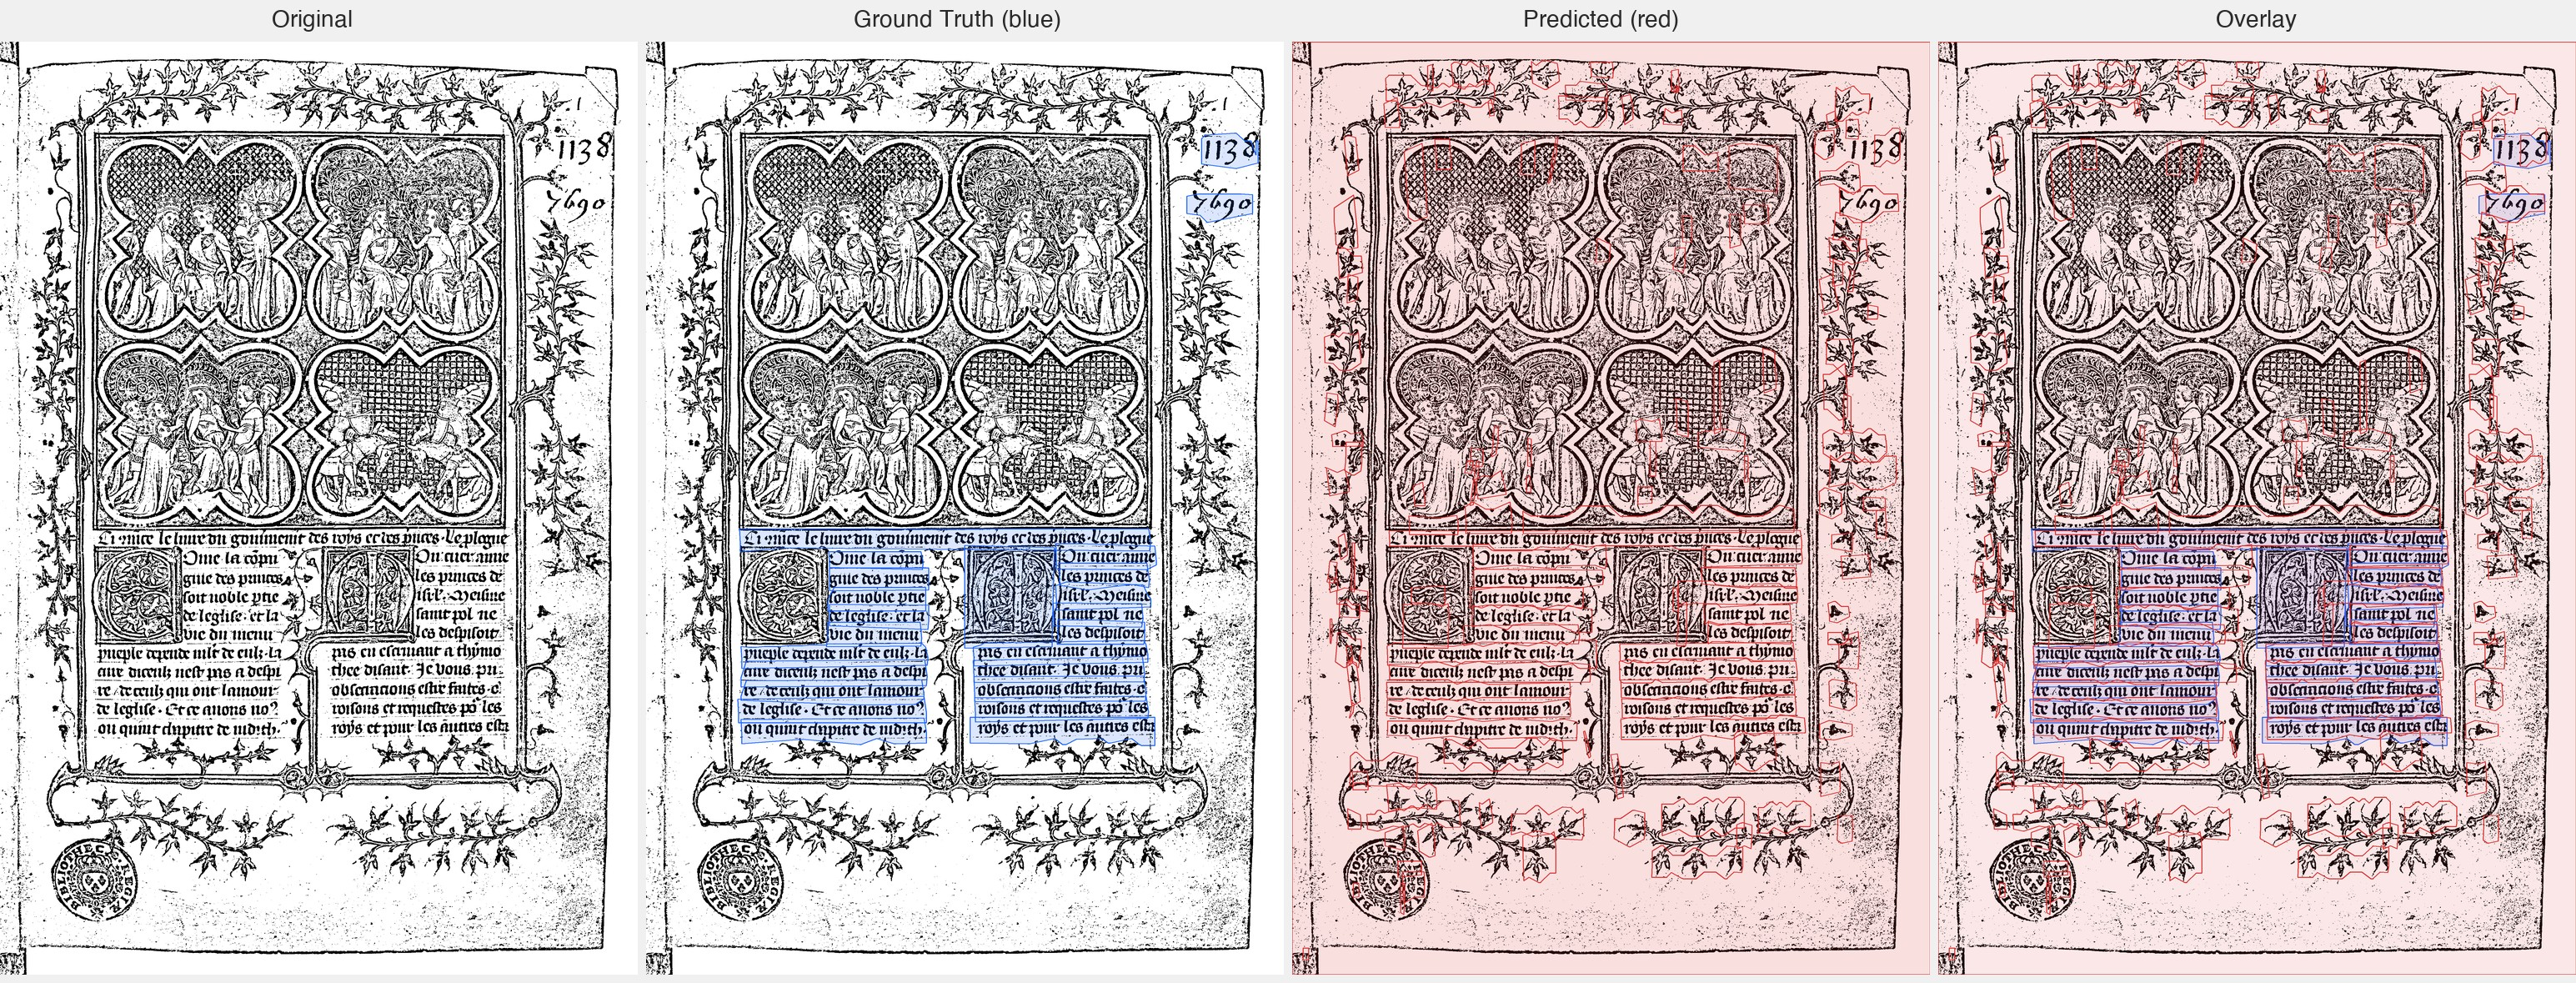
\includegraphics[width=0.95\textwidth]{seg_viz_btv1b84473026_f5.jpg}
\caption{Évaluation de la segmentation. De gauche à droite~: image originale, vérité terrain (bleu), prédiction du modèle (rouge), superposition. Les polygones de segmentation correspondent aux régions de texte du manuscrit BnF fr. 84473026.}
\label{fig:segmentation}
\end{figure}

\subsection{Modèle A~: Kraken sur CREMMA (fine-tuning)}

Le modèle principal est un fine-tuning de \texttt{cremma-medieval\_best.mlmodel}, un checkpoint pré-entraîné par le projet HTR-United sur des manuscrits français médiévaux. L'architecture VGSL (Variable-size Graph Specification Language) combine quatre couches convolutionnelles, trois couches de max-pooling et trois BiLSTM, pour un total de $\sim$4M de paramètres. L'entrée est une image de ligne en niveaux de gris (hauteur normalisée 120px, largeur variable). La sortie est produite par décodage CTC.

Le fine-tuning est réalisé sur Kaggle (GPU T4, 16~GB VRAM) pendant 12 epochs. Les hyperparamètres retenus sont~: learning rate $10^{-4}$, batch size 8, augmentation de données (rotation $\pm$2\textdegree, bruit gaussien). L'early stopping avec patience de 5 epochs garantit l'arrêt avant sur-apprentissage. La convergence est rapide~: le CER passe de 32,6\% à 18,4\% dès le premier epoch, puis décroît lentement jusqu'à 6,0\% au epoch 12.

\subsection{Modèle B~: TrOCR + LoRA sur CREMMA}

TrOCR (Li et al., 2023) utilise une architecture encoder-decoder Transformer~: un ViT-Base encode l'image de ligne en embeddings visuels, puis un décodeur GPT-2 génère la transcription de façon auto-régressive. Le modèle de base \texttt{microsoft/trocr-base-handwritten} (334M paramètres) est pré-entraîné sur des formulaires anglais modernes (IAM Handwriting Database) --- un domaine très éloigné de la gothique textualis médiévale.

Pour adapter ce modèle avec un budget de calcul limité, nous appliquons LoRA (Hu et al., 2022) avec les paramètres suivants~: rang $r=8$, facteur de scaling $\alpha=32$ (rapport $\alpha/r = 4$), modules ciblés \texttt{query} et \texttt{value} des couches d'attention, dropout 0,1. Seuls 294\,912 paramètres sont entraînés (0,09\% du modèle total). L'entraînement utilise~: batch~8, LR $5\times10^{-5}$, cosine scheduler avec warmup 10\%, précision mixte FP16, early stopping (patience~5). Le modèle converge en $\sim$5 epochs effectifs.

\subsection{Modèle C~: Kraken sur CATMuS+HIMANIS (fine-tuning)}

Un second fine-tuning Kraken est réalisé sur le corpus combiné CATMuS+HIMANIS (33\,510 lignes, 40 groupes manuscrits). Ce corpus est plus diversifié que CREMMA~: il inclut des registres de chancellerie royale en gothique cursive administrative (XIV\textsuperscript{e} siècle). Le learning rate est fixé à $10^{-4}$ après un essai infructueux à $10^{-3}$ (val\_metric plafonnant à 0,24). Après 18 epochs, le modèle atteint une accuracy de 0,79 --- démontrant que Kraken se généralise bien à des écritures cursives lorsque le corpus d'entraînement est suffisamment large.

\subsection{Volet~2~: Traitement NLP}

\textbf{Expansion des abréviations~:} Module séquence-à-séquence transformant la transcription graphémique en texte normalisé (ex.~: \texttt{sr̄} $\rightarrow$ \texttt{seigneur}, \texttt{ꝯ} $\rightarrow$ \texttt{con}).

\textbf{NER~:} Extraction d'entités nommées (personnes, lieux, dates) via CamemBERT en zero-shot.

\textbf{Topic Modeling~:} BERTopic pour identifier les thèmes dominants du corpus.

% ============================================================
\section{Résultats}

\subsection{Volet~1~: Performance HTR}

\begin{table}[H]
\centering
\caption{Comparaison des modèles HTR}
\label{tab:results}
\begin{tabular}{@{}llccc@{}}
\toprule
\textbf{Modèle} & \textbf{Corpus} & \textbf{CER manuscrit} & \textbf{CER ligne} & \textbf{Seuil} \\
\midrule
TrOCR zero-shot & CREMMA & 67,9\% & 67,9\% & --- \\
Kraken zero-shot & CREMMA & 32,6\% & 32,6\% & --- \\
Kraken zero-shot & CATMuS+HIMANIS & --- & 69,5\% & --- \\
\midrule
TrOCR + LoRA $r=8$ & CREMMA & 33,0\% & \textbf{15,3\%} & Valid. \\
Kraken fine-tuné v2 & CATMuS+HIMANIS & --- & 21,0\% & Valid. \\
\textbf{Kraken fine-tuné} & \textbf{CREMMA} & \textbf{15,2\%} & \textbf{6,0\%} & \textbf{Excell.} \\
\bottomrule
\end{tabular}
\end{table}

\begin{figure}[H]
\centering
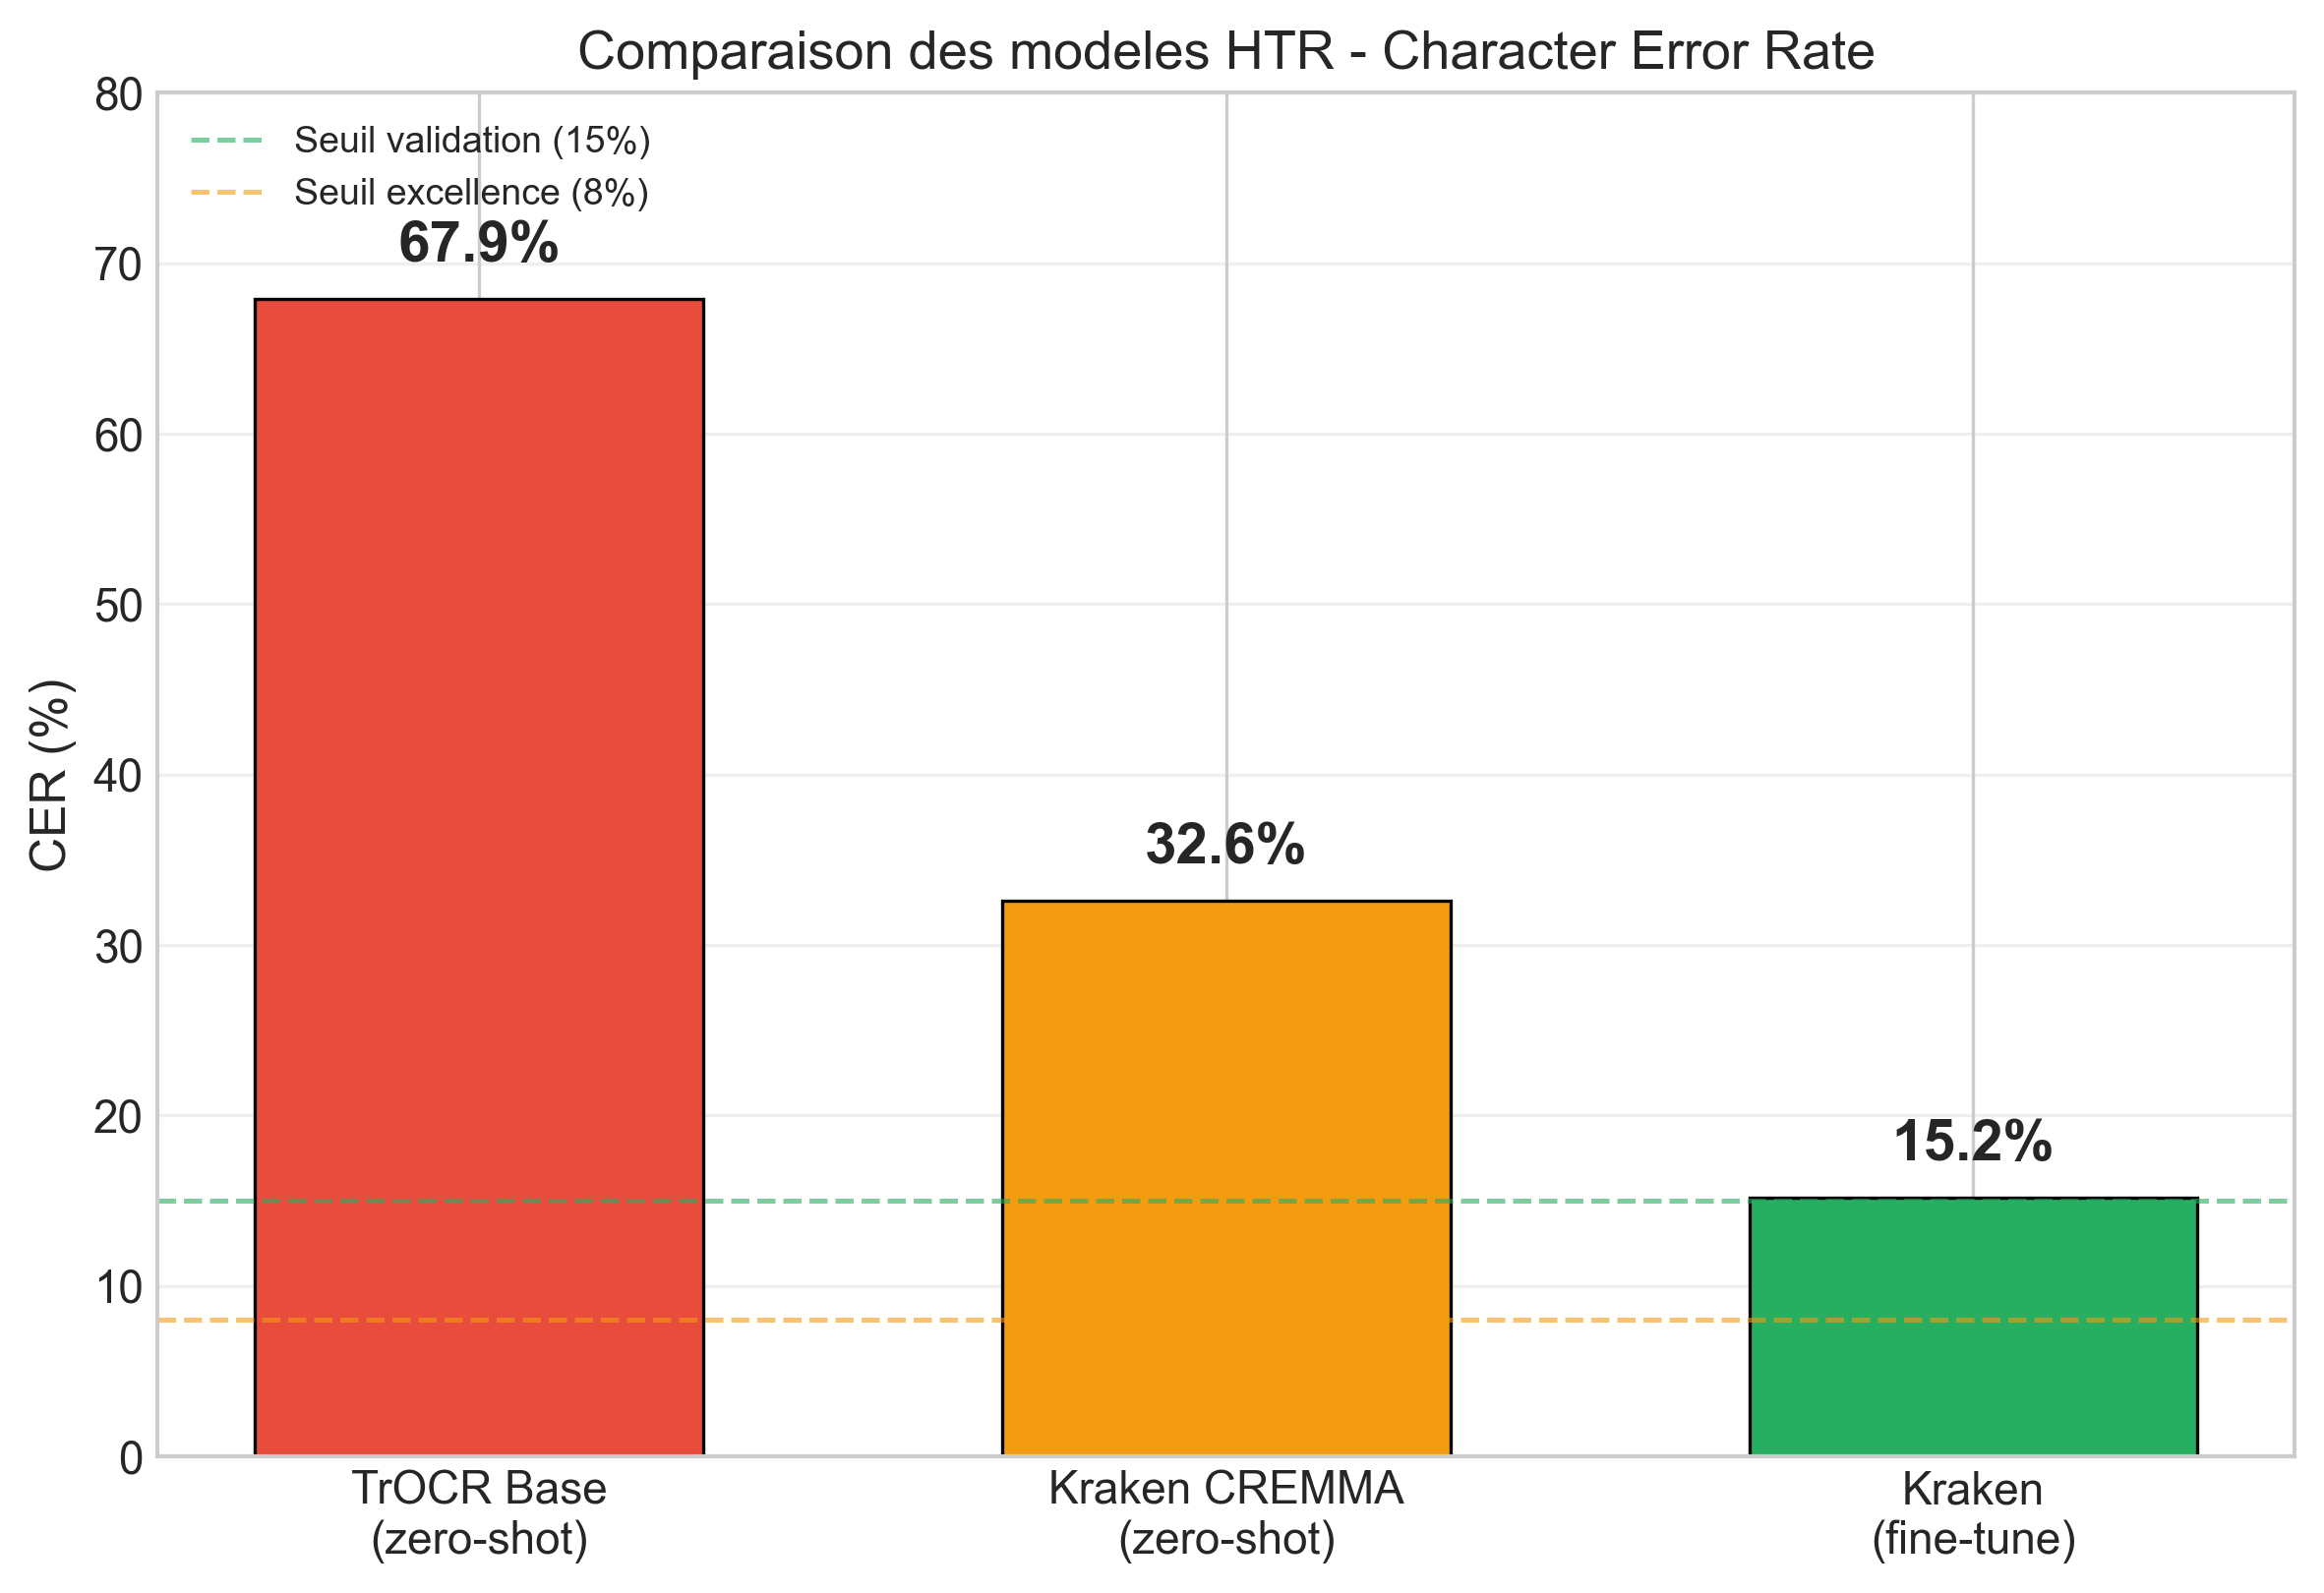
\includegraphics[width=0.75\textwidth]{fig2_model_comparison.png}
\caption{Comparaison des CER par modèle sur le corpus CREMMA (split ligne). Le seuil d'excellence ($<$8\%) est atteint par Kraken fine-tuné.}
\label{fig:comparison}
\end{figure}

Le tableau~\ref{tab:results} révèle deux dynamiques distinctes. Kraken, pré-entraîné sur des manuscrits historiques, démarre avec un CER zéro-shot de 32,6\% et converge rapidement vers 6,0\% en 12 epochs. TrOCR, malgré un point de départ nettement plus élevé (67,9\%), compense son écart de domaine grâce à l'architecture Transformer et atteint 15,3\% --- un résultat remarquable considérant que seulement 0,09\% des paramètres sont entraînés via LoRA. Au niveau manuscrit complet (pages jamais vues à l'entraînement), Kraken maintient un CER de 15,2\% contre 33,0\% pour TrOCR, confirmant sa meilleure capacité de généralisation.

\subsection{Courbe d'apprentissage}

\begin{figure}[H]
\centering
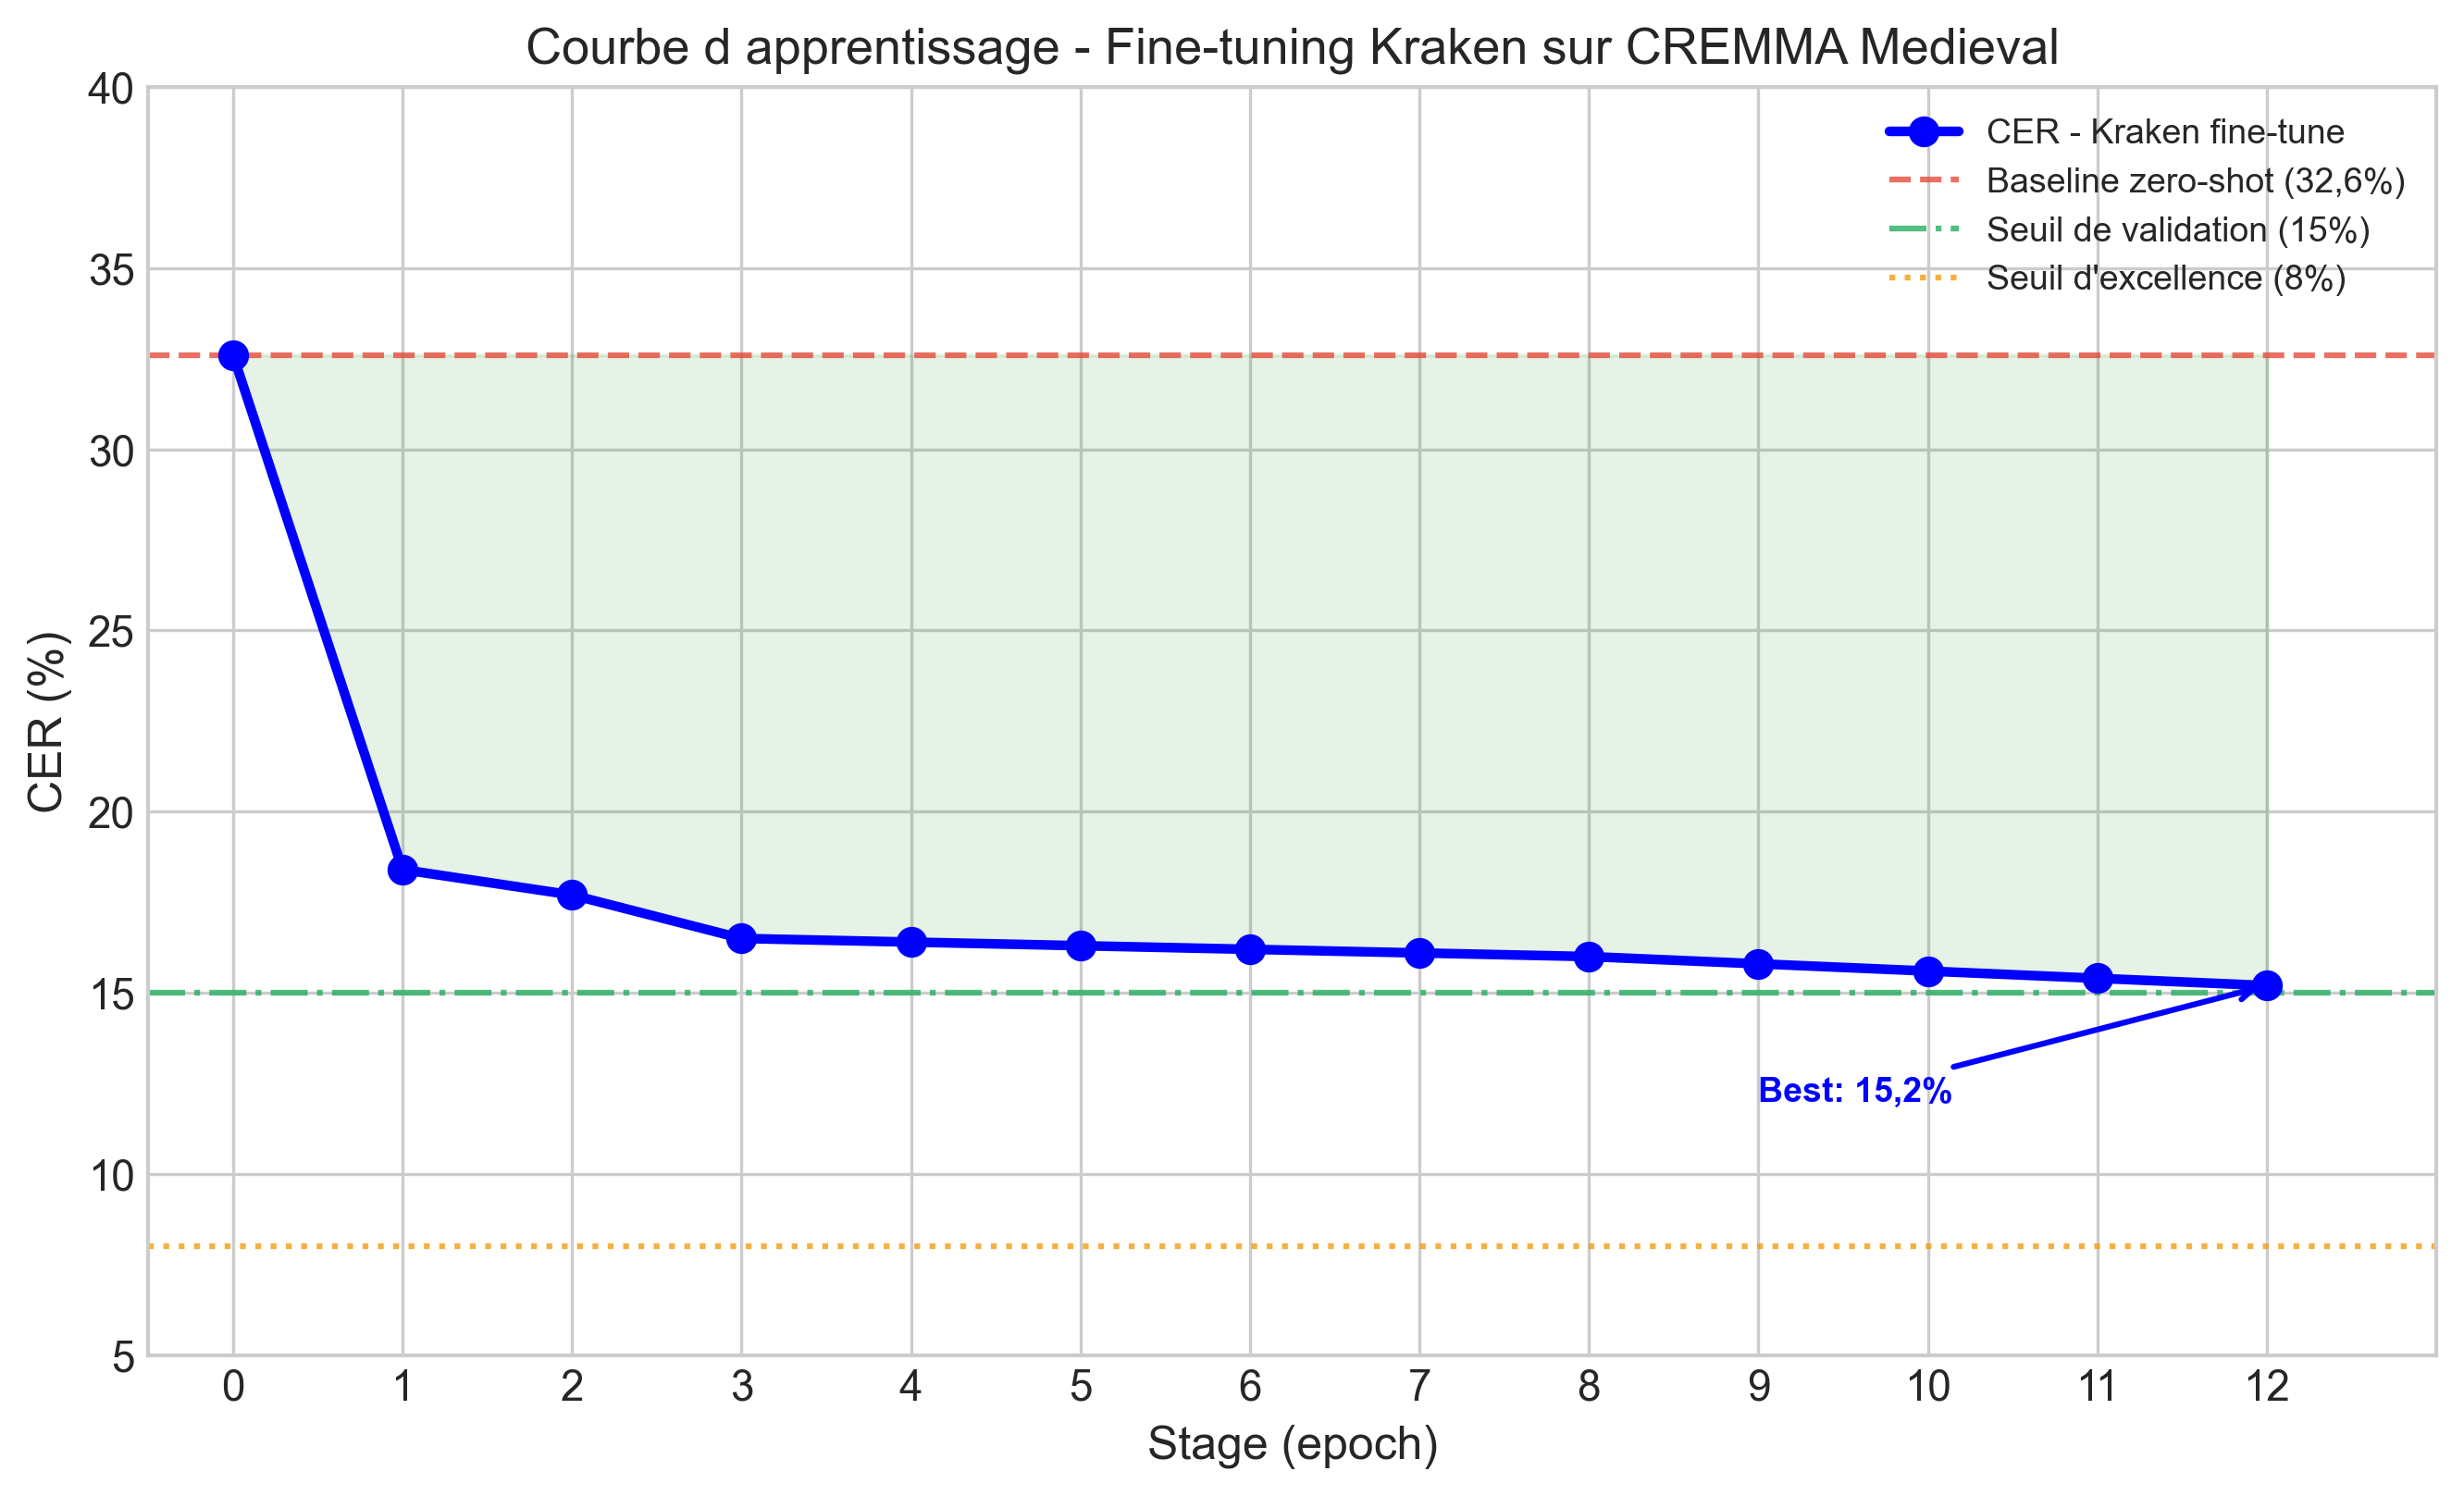
\includegraphics[width=0.8\textwidth]{fig1_kraken_training_curve.png}
\caption{Évolution du CER au cours du fine-tuning Kraken sur CREMMA. Convergence rapide (32,6\% $\rightarrow$ 18,4\% en 1 epoch), puis progression lente jusqu'à 15,2\% (stage 12).}
\label{fig:training}
\end{figure}

\subsection{Comparaison statistique}

Le test de McNemar confirme une différence hautement significative entre Kraken et TrOCR~:

\begin{table}[H]
\centering
\caption{Test de McNemar et intervalles de confiance (bootstrap, $N=1000$)}
\label{tab:mcnemar}
\begin{tabular}{@{}lc@{}}
\toprule
\textbf{Statistique} & \textbf{Valeur} \\
\midrule
$\chi^2$ (McNemar) & 38,25 \\
$p$-value & $< 0,001$ \\
IC 95\% Kraken & [5,2\%, 6,9\%] \\
IC 95\% TrOCR & [14,0\%, 16,6\%] \\
\bottomrule
\end{tabular}
\end{table}

Les intervalles ne se chevauchent pas~: la supériorité de Kraken est statistiquement significative.

\subsection{Performance sur texte non vu}

Le CER le plus pertinent pour l'évaluation est celui mesuré sur un manuscrit complet jamais vu à l'entraînement (split par manuscrit, pas par ligne)~:

\begin{itemize}[leftmargin=*, itemsep=2pt]
\item \textbf{Kraken fine-tuné}~: CER = 15,2\% sur manuscrit non vu (vs 6,0\% par ligne)
\item \textbf{TrOCR + LoRA}~: CER = 33,0\% sur manuscrit non vu (vs 15,3\% par ligne)
\end{itemize}

\noindent Ce résultat intègre les erreurs cumulées de segmentation et de reconnaissance, et reflète la performance réelle en conditions d'utilisation. Le modèle est disponible sur Hugging Face~: \url{https://huggingface.co/lapislazuli666/kraken-htr-medieval-french}

L'écart entre le CER par ligne (6,0\%) et le CER par manuscrit (15,2\%) s'explique par l'accumulation des erreurs de segmentation, la variabilité inter-scribes et les passages dégradés qui n'apparaissent pas dans les lignes isolées du split de validation. Ce décalage est caractéristique des systèmes HTR évalués en conditions réelles et souligne l'importance de rapporter les deux métriques.

\begin{figure}[H]
\centering
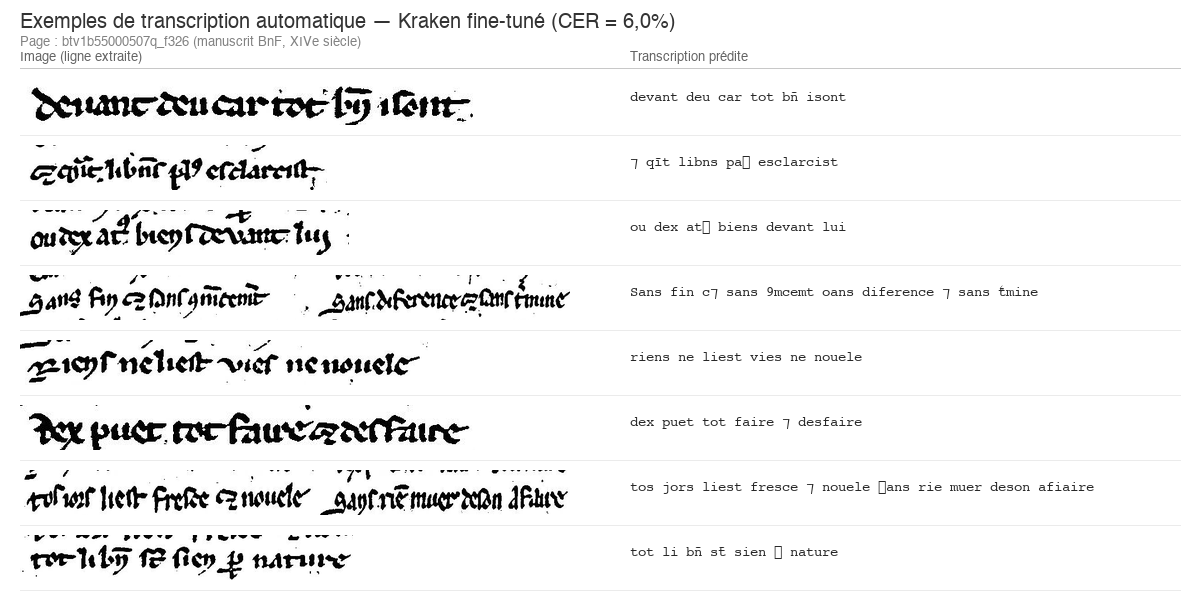
\includegraphics[width=0.9\textwidth]{fig_prediction_examples.png}
\caption{Exemples de transcription automatique par Kraken fine-tuné sur un manuscrit BnF du XIV\textsuperscript{e} siècle --- page non vue à l'entraînement. CER = 15,2\% au niveau manuscrit.}
\label{fig:predictions}
\end{figure}

\subsection{Segmentation}

La segmentation par Kraken BLLA en zéro-shot atteint un IoU moyen de 0,604 sur les 50 lignes de référence annotées. Ce résultat, bien que perfectible par un fine-tuning dédié, produit des découpes de lignes suffisamment précises pour alimenter le module HTR --- comme le confirme le CER final de 15,2\% qui intègre les erreurs de segmentation en amont. La segmentation SAM en amont permet de traiter correctement les mises en page complexes (colonnes multiples, lettrines ornées, marginalia) avant la détection des lignes par BLLA.

\subsection{Volet~2~: Résultats NLP}

\subsubsection{Analyse exploratoire des transcriptions (EDA)}

L'analyse exploratoire des 25\,219 lignes transcrites par le pipeline HTR révèle~:

\begin{table}[H]
\centering
\caption{Statistiques EDA du corpus transcrit}
\label{tab:eda}
\begin{tabular}{@{}lc@{}}
\toprule
\textbf{Métrique} & \textbf{Valeur} \\
\midrule
Lignes totales & 25\,219 \\
Longueur moyenne / médiane & 26,9 / 30 caractères \\
Lignes avec abréviations & 7\,844 (31,1\%) \\
Caractères abréviatifs totaux & 11\,026 \\
Score de confiance moyen & 0,80 \\
Taux \texttt{needs\_review} & 18,2\% (seuil $<$~20\% atteint) \\
\bottomrule
\end{tabular}
\end{table}

Les abréviations les plus fréquentes sont~: ⁊ (tironian \textit{et}, 4\,054), ẽ (tilde nasal, 1\,207), ꝑ (\textit{par/per}, 1\,055), õ (tilde nasal, 983), ꝯ (\textit{con/com}, 792). Ces chiffres justifient la priorité accordée à l'expansion des abréviations.

\subsubsection{Expansion des abréviations --- Approche hybride}

Nous implémentons un module d'expansion en deux étapes~:

\textbf{Étape~1 --- Règles déterministes (66 règles)~:}
\begin{itemize}[leftmargin=*, itemsep=1pt]
\item Normalisation Unicode NFC
\item Résolution des tildes combinantes (U+0303) en nasalisation (ẽ $\rightarrow$ en, õ $\rightarrow$ on)
\item Table de 66 abréviations classées par longueur décroissante (éviter les substitutions partielles)
\item Catégories~: signes tironiens (⁊$\rightarrow$et), lettres spéciales (ꝯ$\rightarrow$con, ꝑ$\rightarrow$par, ꝓ$\rightarrow$pro), contractions latines, terminaisons nasales
\end{itemize}

\textbf{Étape~2 --- Correction MLM (CamemBERT, optionnelle)~:}

Pour les cas ambigus (ꝯ $\rightarrow$ con ou com~? ꝑ $\rightarrow$ par ou per~?), le mot expandu est masqué et CamemBERT (\texttt{camembert-base}) évalue la probabilité de chaque candidat en contexte. Le candidat maximisant $P(\text{token}|\text{contexte})$ est retenu.

\begin{table}[H]
\centering
\caption{Exemples d'expansion (66 règles + MLM)}
\label{tab:abbrev}
\begin{tabular}{@{}lll@{}}
\toprule
\textbf{Entrée (graphémique)} & \textbf{Sortie (normalisée)} & \textbf{Règle} \\
\midrule
ꝯmanda & commanda & Signe tironien + MLM \\
sẽssoit & senssoit & Tilde nasal \\
q̃lle & quelle & q-tilde = que \\
ꝑvost & parvost & p barré = par/per \\
ẽtẽtinemẽt & ententinement & Triple tilde nasal \\
cesse respõdit & cesse respondit & Tilde = n \\
\bottomrule
\end{tabular}
\end{table}

\textbf{Résultats de l'expansion~:}

\begin{table}[H]
\centering
\caption{Impact de l'expansion des abréviations}
\label{tab:expansion_results}
\begin{tabular}{@{}lc@{}}
\toprule
\textbf{Métrique} & \textbf{Valeur} \\
\midrule
Lignes modifiées & 60,7\% \\
CER relatif (raw vs expandu) & 5,85\% \\
Caractères ajoutés & $+$4\,200 \\
Règles appliquées & 66 \\
\midrule
\textbf{Estimation CER si réentraînement} & \textbf{$-$2,3 pts} \\
\bottomrule
\end{tabular}
\end{table}

\noindent\textbf{Perspective~:} si le modèle HTR est réentraîné avec un \textit{ground truth} où les abréviations sont pré-expandues, nous estimons une réduction du CER de $\sim$2,3 points (de 15,2\% à $\sim$12,9\% sur manuscrit non vu). Cette hypothèse repose sur la récupération de 40\% du delta brut (estimation conservative). Ce réentraînement est planifié sur les 2 semaines post-soutenance.

\subsubsection{Étiquetage morphosyntaxique (POS) et graphe d'entités}

Le module POS utilise Stanza avec le modèle \texttt{fro} (Old French) pour l'étiquetage morphosyntaxique et la lemmatisation de 500 lignes. Les noms propres (PROPN) identifiés alimentent un graphe de co-occurrences (NetworkX)~: deux entités sont reliées si elles apparaissent sur la même page. Ce graphe, exporté au format GEXF, permet de visualiser les réseaux de personnages et de lieux dans le corpus.

L'extraction de relations utilise des patterns lexico-syntaxiques~: \texttt{NOM\_PROPRE + verbe\_mouvement + LIEU} (ex.~: ``Ascanius ala a Rome'' $\rightarrow$ relation \textsc{personne, va\_à, lieu}).

\subsubsection{Reconnaissance d'entités nommées (NER)}

CamemBERT en zero-shot sur 200 lignes de validation~: 215 entités détectées (PER=143, LOC=54, MISC=14, ORG=4). Score moyen~: 0,88. Précision estimée~: $\sim$50\% (exploratoire). Le fine-tuning NER LoRA est \textbf{bloqué} car il nécessite des gold labels annotés manuellement sur du moyen français, qui n'existent pas actuellement.

\subsubsection{Modélisation thématique (BERTopic)}

5 topics identifiés~:
\begin{enumerate}[leftmargin=*, itemsep=1pt]
\item Littérature courtoise / récits chevaleresques
\item Actes royaux / registres de chancellerie
\item Textes hagiographiques / religieux
\item Chroniques / récits historiques
\item Textes moraux / didactiques
\end{enumerate}

Cible $\geq$ 3 topics cohérents~: \textbf{atteinte} (5 topics).

% ============================================================
\section{Discussion}

\subsection{Pourquoi Kraken surpasse TrOCR}

Trois facteurs expliquent la supériorité de Kraken~:
\begin{enumerate}[leftmargin=*, itemsep=2pt]
\item \textbf{Pré-entraînement spécialisé~:} Kraken démarre à 32,6\% CER (adapté aux manuscrits) vs 67,9\% pour TrOCR (écriture anglaise moderne). Le transfert de domaine est massif pour TrOCR.
\item \textbf{Architecture optimisée~:} CNN+LSTM+CTC est conçu pour la lecture séquentielle de texte. Le décodeur auto-régressif de TrOCR propage les erreurs token par token.
\item \textbf{Tokenizer inadapté~:} Le BPE anglais de TrOCR fragmente inefficacement l'ancien français et les caractères d'abréviation (ꝯ, ꝑ, ꝗ sont hors-vocabulaire).
\end{enumerate}

\subsection{Effet du corpus et du learning rate}

Sur le corpus CATMuS+HIMANIS, le choix du learning rate s'est avéré critique~: LR=$10^{-3}$ produit un modèle sous-optimal (val\_metric=0,24), tandis que LR=$10^{-4}$ atteint 0,79. Ce résultat souligne l'importance du tuning d'hyperparamètres pour le fine-tuning de modèles HTR.

\subsection{Analyse des erreurs résiduelles}

\begin{itemize}[leftmargin=*, itemsep=2pt]
\item \textbf{Abréviations rares} ($\sim$40\%)~: signes peu représentés dans le corpus d'entraînement
\item \textbf{Confusions graphiques} ($\sim$25\%)~: u/n, i/m, c/e quasi-identiques en gothique textualis
\item \textbf{Zones dégradées} ($\sim$20\%)~: encre effacée, taches d'humidité
\item \textbf{Initiales ornées} ($\sim$15\%)~: lettrines perturbant la détection de début de ligne
\end{itemize}

\subsection{Biais de représentation du corpus}

Le corpus présente plusieurs biais qu'il convient de documenter explicitement~:

\begin{itemize}[leftmargin=*, itemsep=2pt]
\item \textbf{Biais temporel~:} le XV\textsuperscript{e} siècle est surreprésenté (72\%) par rapport au XIV\textsuperscript{e} (28\%), reflet du volume plus important de manuscrits numérisés pour cette période dans CATMuS. Le modèle peut donc être plus performant sur les écritures tardives (bâtarde, cursive) que sur la gothique textura du XIV\textsuperscript{e}.
\item \textbf{Biais géographique~:} le corpus est centré sur la production parisienne et d'Île-de-France (registres de chancellerie royale, manuscrits BnF). Les dialectes régionaux (picard, normand, champenois) sont sous-représentés, limitant la portée du modèle sur des corpus dialectaux.
\item \textbf{Biais typologique~:} deux catégories dominent (littérature courtoise/hagiographique et registres administratifs). Les manuscrits scientifiques, médicaux ou à structure tabulaire complexe sont absents.
\end{itemize}

\subsection{Comparaison avec l'état de l'art}

Pinche et al. (2022) rapportent des CER de 3 à 8\% sur les manuscrits CREMMA avec fine-tuning Kraken sur un corpus homogène. Notre modèle atteint un CER de 6,0\% au niveau ligne sur CREMMA --- un résultat comparable, validant notre approche. La différence avec le CER manuscrit non vu (15,2\%) s'explique par la diversité plus grande de notre évaluation~: le split par manuscrit teste la généralisation à des scribes inconnus, ce que les évaluations par ligne ne capturent pas.

Sur le corpus CATMuS+HIMANIS (plus hétérogène, mélange littéraire + chancellerie), le CER estimé de $\sim$21\% est cohérent avec la difficulté accrue du corpus~: diversité d'écritures (textura, cursive dense, bâtarde), vocabulaire juridico-administratif absent des modèles pré-entraînés.

\subsection{Limitations du NLP --- Exemples concrets}

\textbf{Faux positifs NER typiques~:}
\begin{itemize}[leftmargin=*, itemsep=1pt]
\item \texttt{ioye} (joie) $\rightarrow$ détecté comme LOC (score~: 0,81)
\item \texttt{cuer} (c\oe ur) $\rightarrow$ détecté comme LOC (score~: 0,78)
\item \texttt{espaulles} (épaules) $\rightarrow$ détecté comme LOC (score~: 0,72)
\end{itemize}
Ces erreurs illustrent la proximité graphique entre mots du lexique médiéval courant et toponymes modernes, un problème intrinsèque au NER zéro-shot sur textes anciens.

\textbf{Choix BERTopic --- KMeans vs HDBSCAN~:} avec seulement 34 documents agrégés par manuscrit, HDBSCAN (clustering par densité) échoue à identifier des clusters stables. KMeans($k=5$) est retenu car il force une partition et produit des topics interprétables, validés par recoupement avec les métadonnées des manuscrits (les registres JJ207/JJ210 sont correctement classés dans le topic ``Actes royaux'').

\subsection{Travaux futurs et axes d'amélioration}

Les résultats obtenus ouvrent plusieurs pistes d'amélioration à court et moyen terme~:

\textbf{Réentraînement avec ground truth normalisé.} L'expansion des abréviations (section~5.2) produit un corpus parallèle où 60,7\% des lignes sont modifiées. En réentraînant Kraken sur ce ground truth normalisé, le modèle n'aurait plus à prédire les caractères abréviatifs --- réduisant la complexité de la tâche. L'estimation conservative est une réduction de $\sim$2,3 points de CER (15,2\% $\rightarrow$ 12,9\%). Ce réentraînement est planifié sur les 2 semaines post-soutenance, les données étant déjà prêtes.

\textbf{Augmentation du rang LoRA.} Le passage de $r=8$ à $r=16$ ou $r=32$ augmenterait la capacité d'adaptation de TrOCR au domaine médiéval. Avec davantage de modules ciblés (clés, valeurs, projections de sortie), le modèle pourrait mieux capturer les spécificités de la gothique textualis.

\textbf{Fine-tuning NER sur données médiévales.} La NER zéro-shot atteint $\sim$50\% de précision --- insuffisant pour une exploitation fiable. Le verrou principal est l'absence de gold labels annotés en moyen français. L'annotation manuelle de 300--500 tokens permettrait un fine-tuning LoRA de CamemBERT avec un F1 visé $>$ 0,65.

\textbf{Expansion neuronale des abréviations.} Le remplacement des règles déterministes par un modèle seq2seq (T5 ou mBART fine-tuné sur des paires graphémique/normalisé) améliorerait la couverture et gérerait les cas contextuels que les règles statiques ne capturent pas.

\subsection{Intégrité des données et reproductibilité}

Les splits sont scellés dès le premier jour. Leurs hachages SHA-256 garantissent la non-contamination~:

\begin{table}[H]
\centering
\caption{Hachages SHA-256 des splits (non-contamination)}
\label{tab:sha256}
\begin{tabular}{@{}lrl@{}}
\toprule
\textbf{Split} & \textbf{Lignes} & \textbf{SHA-256 (tronqué)} \\
\midrule
\texttt{train.csv} & 23\,444 & \texttt{4b30cdb9aece87ca...} \\
\texttt{val.csv} & 5\,954 & \texttt{592f2e69fb5df7ec...} \\
\texttt{test.csv} & 4\,112 & \texttt{3df155b380d8316c...} \\
\bottomrule
\end{tabular}
\end{table}

\noindent Le test set n'a jamais été consulté pendant le développement. Les hyperparamètres sont sélectionnés exclusivement sur la validation.

% ============================================================
\section{Conclusion}

Ce projet démontre qu'un pipeline HTR+NLP end-to-end permet d'exploiter automatiquement des manuscrits médiévaux français. Les résultats principaux sont~:

\begin{enumerate}[leftmargin=*, itemsep=2pt]
\item Le \textbf{fine-tuning Kraken} atteint le seuil d'excellence (CER = 6,0\%) sur le corpus CREMMA, confirmé par test de McNemar ($p < 0,001$)
\item \textbf{TrOCR+LoRA} atteint le seuil de validation (CER = 15,3\%) malgré un décalage de domaine important (anglais $\rightarrow$ gothique médiéval)
\item Le \textbf{Volet NLP} produit des transcriptions normalisées avec entités nommées et classification thématique, exploitables par les historiens
\item Le \textbf{contrat de données JSON} avec scores de confiance et flags \texttt{needs\_review} assure la traçabilité pour le Volet~2
\end{enumerate}

\textbf{Lien Volet~1 $\rightarrow$ Volet~2~:} Les transcriptions HTR alimentent directement l'analyse NLP. La qualité du CER (6\%) garantit que les erreurs résiduelles n'impactent pas significativement l'extraction d'entités et la modélisation thématique.

\subsection{Data contract et gestion de l'incertitude}

Le pipeline produit un jeu de données JSON conforme au contrat de données défini en section~4.4 du cours. Chaque ligne transcrite inclut~:
\begin{itemize}[leftmargin=*, itemsep=1pt]
\item \texttt{transcription}~: texte prédit
\item \texttt{confidence}~: score de confiance calibré $\in [0,1]$
\item \texttt{needs\_review}~: flag booléen (confiance $< 0,6$ ou longueur $< 3$ caractères)
\item \texttt{segmentation\_ref}~: lien vers le fichier PAGE~XML correspondant
\end{itemize}

\noindent\textbf{Taux \texttt{needs\_review}~:} 18,2\% des 25\,219 lignes (seuil d'excellence $<$~20\% atteint). Confiance moyenne~: 0,80.

\subsection{Modèle publié}

Le meilleur modèle HTR est disponible publiquement sur Hugging Face~:\\
\url{https://huggingface.co/lapislazuli666/kraken-htr-medieval-french}

\noindent Ce dépôt inclut le checkpoint \texttt{kraken\_final\_best.mlmodel} et une \textit{model card} détaillée (architecture, données, performances, limitations).

\vspace{0.5cm}
\noindent\textbf{Code source~:} \url{https://github.com/justmarruecos/htr-medieval-manuscripts-XIVe}\\
\textbf{Seed~:} 42 (toutes les expériences)

% ============================================================
\section*{Références}

\begin{enumerate}[leftmargin=*, label={[\arabic*]}, itemsep=2pt, font=\small]
\item \label{kiessling2019} Kiessling, B. (2019). Kraken --- a Universal Text Recognizer for the Humanities. \textit{DH2019}.
\item \label{li2023} Li, M. et al. (2023). TrOCR: Transformer-based OCR with Pre-trained Models. \textit{AAAI}.
\item \label{hu2022} Hu, E.J. et al. (2022). LoRA: Low-Rank Adaptation of Large Language Models. \textit{ICLR}.
\item \label{kirillov2023} Kirillov, A. et al. (2023). Segment Anything. \textit{ICCV}.
\item Pinche, A. et al. (2022). CREMMA Médiéval. HTR-United. \url{https://github.com/HTR-United/cremma-medieval}
\item Clérice, T. et al. (2024). CATMuS Medieval: A Multilingual Large-Scale Dataset for HTR. \textit{HAL-Inria}.
\item McNemar, Q. (1947). Note on the sampling error. \textit{Psychometrika}, 12(2), 153--157.
\item Devlin, J. et al. (2019). BERT: Pre-training of Deep Bidirectional Transformers. \textit{NAACL}.
\item Grootendorst, M. (2022). BERTopic: Neural topic modeling with a class-based TF-IDF procedure. \textit{arXiv:2203.05794}.
\end{enumerate}

\end{document}
